% \section{Preliminary}
% \label{sec:preliminary}

% \textbf{Ladder Side Tuning}\cite{sung2022lst} trains a ladder side network, a small and separate network that takes intermediate activations from the backbone transformer as input and makes predictions. It includes a downward projection $h_i^f=x_iW_d^T$ to decrease dimension of the feature and a gated connection to integrate the intermediate activation of the backbone $f$ and the features of the side network $g$ Adaptively. The output is calculated by
% \begin{equation}
%     \boldsymbol{h}_{i}^{g}=\Phi(\mu_{i} * \boldsymbol{h}_{i}^{f}+\left(1-\mu_{i}\right) * \boldsymbol{h}_{i-1}^{g})
% \end{equation}
% where $\mu_{i}=\operatorname{sigmoid}\left(\frac{\alpha_{i}}{T}\right)$ is a gate parameterized with a learnable zero-initialized scalar $\alpha_i$ and temperature $T$(= 0.1), $\Phi$ is a linear layer that projects the fused features.

% \textbf{Prompt tuning}\cite{li2021prefix,jia2022visual} freezes the backbone network during fine-tuning while inserting learnable tokens into the input token sequence. Prompt tokens interact with the original tokens through attention mechanisms. Given the class token $x_{cls}\in R^{1 
% \times d}$ and patch tokens $T \in R^{N \times d}$, where $N$ is the num of patch tokens, we can insert prompt tokens $P_i \in R^{n \times d}$ for each layer following VPT-Deep\cite{jia2022visual}, where $n \ll N$ is the num of prompt tokes.The output of $i$-th layer($L(\cdot)$) is expressed as follows:
% \begin{equation}
%     \boldsymbol{x}_{i}=L_{i}\left(\left[\boldsymbol{T}_{c l s} ; \boldsymbol{P}_{i} ; \boldsymbol{T}\right]\right)
% \end{equation}

\begin{figure*}
    \centering
    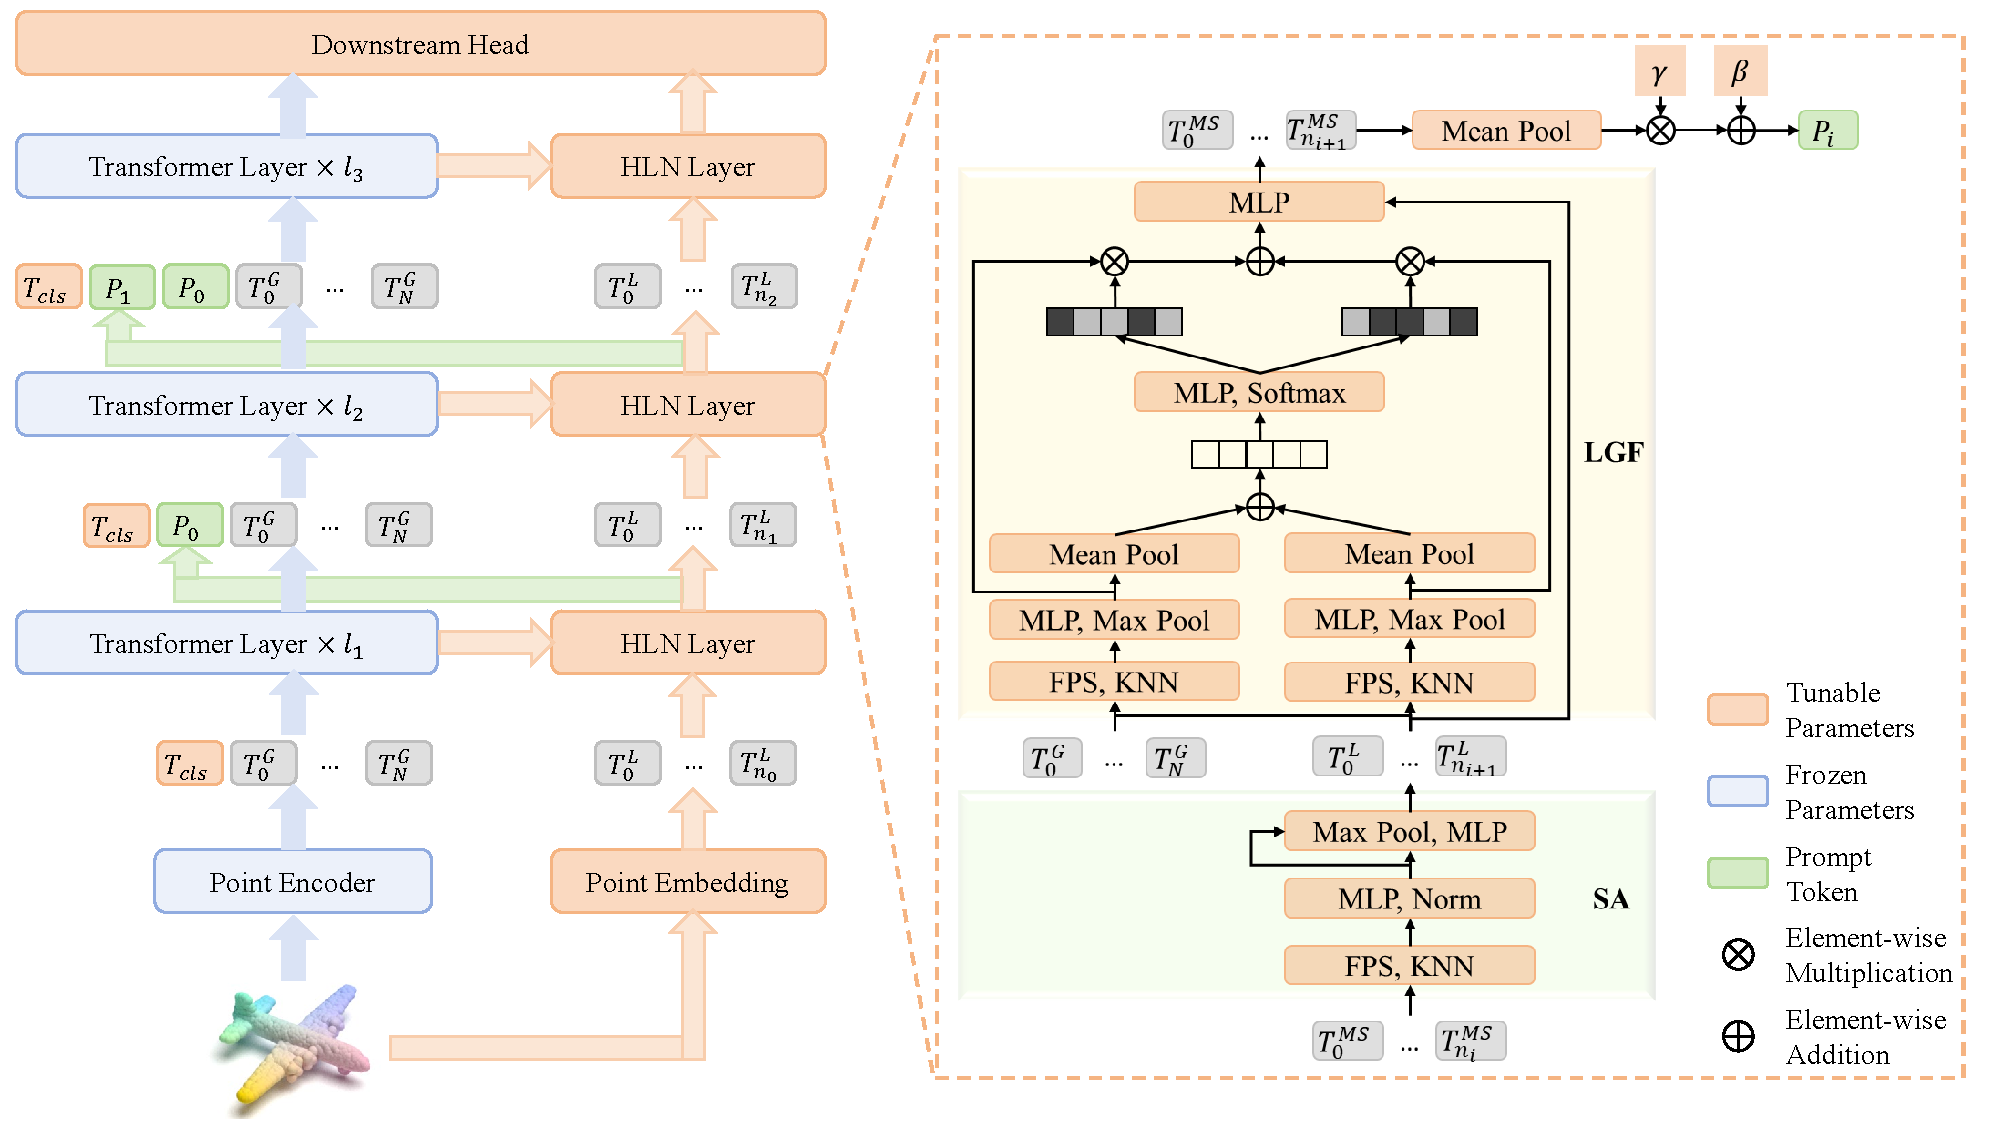
\includegraphics[width=\linewidth]{fig/Overall.pdf}
    \caption{The overall of our PLT. During fine-tuning, we froze the pre-trained backbone network and only fine-tune the PLT branch and the class token. The PLT branch consists of two main components: 1) Set Abstraction (SA), and 2) Local-Global Fusion Module (LGF).
}
    \label{fig:overall}
\end{figure*}

\section{Methodology}
\label{sec:methodology}

%Fine-tuning pre-trained models, though effective across domains, often incurs high computational and storage costs. To address this, We propose Point Ladder Tuning (PLT), an efficient fine-tuning method for 3D point cloud learning that combines LST~\cite{sung2022lst} and prompt tuning\cite{jia2022visual}. PLT optimizes parameter efficiency and task performance by integrating both local and global features, addressing LST’s limitations in capturing local features and prompt tuning’s lack of adaptability across instances.

\lr{To enable effective cross-domain fine-tuning of pre-trained models while mitigating the high computational and storage costs associated with full-parameter updates, we propose Point Ladder Tuning (PLT), a parameter-efficient fine-tuning framework for 3D point cloud learning. PLT hierarchically integrates ladder connections into frozen layers of the pre-trained model and employs task-specific prompts to guide the model’s behavior without modifying its original parameters. PLT enhances parameter efficiency and task performance by jointly leveraging local and global feature representations, thereby overcoming two key limitations: (1) the inability of Ladder Side-Tuning (LST) to effectively capture fine-grained local features, and (2) the limited instance-level adaptability of conventional prompt tuning methods.}

%combines LST~\cite{sung2022lst} and prompt tuning\cite{jia2022visual}. 

%PLT optimizes parameter efficiency and task performance by integrating both local and global features, addressing LST’s limitations in capturing local features and prompt tuning’s lack of adaptability across instances.


Thus, we introduces a hierarchical Ladder network (HLN) that directly extracts local features from the input point cloud and fuses them with the global activations of the backbone network to create multi-scale representations. The HLN consists of two main components: (1) a set abstraction (SA) module, detailed in Sec.~\ref{sec:HLN}, and (2) a Local-Global Fusion (LGF) module, discussed in Sec.~\ref{sec:LGF}. 
Further, dynamic prompt tokens generated from these fused features refine the backbone’s global features, achieving high task-specific performance with minimal parameter updates, which is described in Sec.~\ref{sec:FT_backbone}. This approach thus maintains the semantic richness of pre-trained models while substantially reducing computational demands, demonstrating effectiveness across point cloud applications like semantic segmentation.
Our framework is shown in Fig.~\ref{fig:overall2}.

\subsection{Hierarchical Ladder Network}
\label{sec:HLN}
Pre-trained models primarily capture global information from input point clouds through attention mechanisms; however, they often overlook local features, which are essential for downstream tasks, particularly dense prediction. Although PointPEFT~\cite{tang2024point} introduces a Geometry-Aware Adapter to enhance local feature learning, it still relies heavily on the global intermediate activations of pre-trained models, limiting its ability to effectively capture intrinsic local features from the original point cloud. Furthermore, since most pre-trained models operate at a single scale, they lack the multi-scale information necessary for optimal performance in downstream tasks.

To address these limitations, we propose a Hierarchical Ladder Network (HLN) to capture local information across multiple scales within the input point cloud. The HLN module includes multiple layers designed to capture features at varying scales, and our experiments validate its effectiveness. The HLN layer consists of two key components: (1) Set Abstraction (SA) and (2) Local-Global Fusion (LGF) module. 
In this section, we introduce SA, with LGF discussed further in Sec.~\ref{sec:LGF}.

Given an input point cloud $P \in \mathbb{R}^{N \times 3}$, where $N$ is the number of points, we first apply point embedding to map $P$ into a high-dimensional space, resulting in a point cloud feature matrix $F \in \mathbb{R}^{N \times C}$, where $C$ represents the feature dimension. We then use Set Abstraction (SA) for downsampling, starting with farthest point sampling (FPS) to select a set of center points $C=\{c_1, \ldots, c_n\}$. Next, k-nearest neighbors (KNN) constructs local neighborhoods $P(c)=\{p^1_c, \ldots, p^k_c\}$ and $F(c)=\{f^1_c, \ldots, f^k_c\}$ for each center point $c$. Finally, max pooling and a multi-layer perceptron (MLP) produce the output point cloud features, as defined by the following equations:
\begin{flalign}
	\boldsymbol{f}_{c} & = \varphi \left(\left[\boldsymbol{f}_{c}^{j} ;\left(\boldsymbol{p}_{c}-\boldsymbol{p}_{c}^{j}\right)\right]\right)\\
	\boldsymbol{f}_{c}^{'} & = \boldsymbol{f}_{c} + \rho \left( h_{\boldsymbol{\Theta}}\left ( \boldsymbol{f}_{c} \right) \right)
\end{flalign}
where $\rho$ and $\varphi$ denote MLPs, $[\cdot, \cdot]$ indicates the concatenation operation, and $h_{\boldsymbol{\Theta}}$ represents the aggregation function. Unless otherwise specified, max pooling is used.

\subsection{Local-Global Fusion Module}
\label{sec:LGF}
To effectively leverage the local features captured in the PLT branch alongside the global features from the pre-trained backbone, we introduce a Local-Global Fusion (LGF) module that adaptively combines both types of information via selective attention. Given an input point cloud $P_{s}$ with corresponding features $F_{s}$ from the HLN layer, and an output point cloud $P_{m}$ with features $F_{m}$ from the backbone network, we first map the backbone features to match the dimensionality of the HLN layer’s feature vectors using a learnable matrix $W$:
\begin{equation}
	\boldsymbol{F}_{m}^{'} = \boldsymbol{F}_mW 
\end{equation}

We then perform Set Abstraction (SA) operations to extract global features $F_g$, which represent interactions between $P_s$ and $P_m$, and local features $F_l$, derived from the interactions within $P_s$ in the HLN layer.

To fuse these global and local features, we employ a selective attention mechanism. This mechanism allows the model to focus adaptively on the most relevant information from each feature source, ensuring both global context and local details are integrated. First, we apply an aggregation function $\mathcal{A}$, typically average pooling, to obtain global and local feature vectors:
\begin{equation}
	\boldsymbol{f}_g, \boldsymbol{f}_l = \mathcal{A}(\boldsymbol{F}_g),  \mathcal{A}(\boldsymbol{F}_l)
\end{equation}

These global and local features are then summed and passed through an MLP to produce representations $z_g$ and $z_l$:
\begin{equation}
	\boldsymbol{z}_g, \boldsymbol{z}_l = \alpha \left( \boldsymbol{f}_g + \boldsymbol{f}_l \right)
\end{equation}
where $\alpha$ represents an MLP.

Using Softmax, we compute attention weights $s_g$ and $s_l$ for the global and local features:
\begin{equation}
	\boldsymbol{s}_g^i = \frac{e^{\boldsymbol{z}_g^i}}{e^{\boldsymbol{z}_g^i} + e^{\boldsymbol{z}_l^i}}, \quad \boldsymbol{s}_l^i = \frac{e^{\boldsymbol{z}_l^i}}{e^{\boldsymbol{z}_g^i} + e^{\boldsymbol{z}_l^i}}
\end{equation}

The fused multi-scale features are then computed as the weighted sum of the global and local features:
\begin{equation}
	\boldsymbol{F}_{ms} = \boldsymbol{s}_g \boldsymbol{F}_g + \boldsymbol{s}_l \boldsymbol{F}_l
\end{equation}

Finally, an MLP $\tau$ performs feature mapping, and the output is added to the input features to produce the final fused output:
\begin{equation}
	\boldsymbol{F}_{o} = \boldsymbol{F}_s + \tau \left( \boldsymbol{F}_{ms} \right)
\end{equation}

By adaptively emphasizing the most relevant local and global features, our LGF module effectively integrates multi-scale information, enhancing the model's capacity to capture both fine-grained details and broad structural context in point clouds—particularly valuable for dense prediction tasks.

\subsection{Fine-tuning on the Backbone Network}
\label{sec:FT_backbone}
To enable the pre-trained backbone network to produce enhanced global features tailored for downstream tasks, we propose a dynamic prompt generation method based on the multi-scale point cloud feature output $F_{o}$ from the LGF module. First, $F_{o}$ is mean-pooled to obtain a compact representation. This pooled feature is then scaled and shifted using learnable parameters $\gamma$ and $\beta$, generating a multi-scale prompt $p$. To maximize parameter efficiency, we reuse $W$ to align the dimensionality of the multi-scale prompts with that of the backbone network features. The formula for this process is as follows:
\begin{equation}
	p = \left( \boldsymbol{\gamma} \times \frac{1}{n}\sum_i^n{\boldsymbol{F}_{o}^i} + \boldsymbol{\beta} \right) W^T
\end{equation}
where $n$ is the number of tokens in $F_o$.

Finally, the multi-scale prompts are incorporated into the backbone network during training. The output of the $l$-th transformer layer, $x_l$, is given by:
\begin{equation}
	\boldsymbol{x}_l = L_l\left(\left[\boldsymbol{T}_{cls} ; \boldsymbol{p}_{0}, \ldots, \boldsymbol{p}_{i-1} ; \boldsymbol{T}\right]\right)
\end{equation}

To further enhance performance, we follow SSF~\cite{lian2022scaling} and apply scaling and shifting to the output of each module within the backbone network, enabling the extraction of task-specific global information. Given an input $x$, the output $y$ is calculated as:
\begin{equation}
	\boldsymbol{y} = \boldsymbol{s} \times \boldsymbol{x} + \boldsymbol{t}
\end{equation}
where $s$ and $t$ are learnable scaling and shifting parameters, respectively.


